\documentclass[../../main.tex]{subfiles}
\graphicspath{{../../image/}{../../figure/}}
\begin{document}

\section{非线性潜变量模型}\label{section:ch16-非线性潜变量模型}

到目前为止，在本章中，我们关注的是基于从潜空间到数据空间的线性变换的潜变量模型。自然地，我们会问：是否可以利用深度神经网络的灵活性来表示更复杂的变换，同时利用深度神经网络的学习能力让得到的分布适配于一个数据集？

考虑一个简单的向量变量 $\bm{z}$ 上的分布，例如高斯分布：
\begin{align}
p(\bm{z})=\mathcal{N}(\bm{z}|\bm{0},\bm{I})
\label{align:ch16-nl-prior}
\end{align}

假设我们使用一个由深度神经网络给出的函数 $\bm{x}=\bm{g}(\bm{z},\bm{w})$ 来变换 $\bm{z}$，其中 $\bm{w}$ 代表权重和偏置。$\bm{z}$ 上的分布与神经网络的结合定义了 $\bm{x}$ 上的分布。从这样的模型中采样是直截了当的，因为我们可以从 $p(\bm{z})$ 中生成样本，然后使用神经网络函数对每个样本进行变换，以获得对应的 $\bm{x}$ 的样本。这是一个高效的过程，因为它不涉及迭代。

\subsection{非线性流形}\label{subsection:ch16-非线性流形}

要求潜空间和数据空间具有相同的维度是一个重大的限制。考虑这样一种情况：$\bm{z}$ 的维度是 $M$，$\bm{x}$ 的维度是 $D$，其中 $M<D$。在这种情况下，$\bm{x}$ 上的分布局限于维度为 $M$ 的流形或子空间。许多机器学习应用中都出现了低维流形，例如在模拟自然图像的分布时。非线性潜变量模型（nonlinear latent variable model）在建模此类数据时可能非常有用，因为它们表达了强烈的归纳偏置，即数据并不"填满"数据空间，而是被限制在一个流形上，尽管这个流形的形状和维度通常是未知的。

为了从数据中学习 $\bm{g}(\bm{z},\bm{w})$，考虑如何计算似然函数 $p(\bm{x}|\bm{w})$。$\bm{x}$ 上的分布由密度的变量变换公式给出：
\begin{align}
p(\bm{x})=p(\bm{z}(\bm{x}))\,|\det \bm{J}(\bm{x})|
\label{align:ch16-change-var}
\end{align}
其中 $\bm{J}$ 是偏导数的雅可比矩阵。

要计算式\eqref{align:ch16-change-var}右侧的分布 $p(\bm{z}(\bm{x}))$（对于给定的数据向量 $\bm{x}$）和同一点的雅可比矩阵，我们需要使用神经网络函数的逆函数 $\bm{z}=\bm{g}^{-1}(\bm{x},\bm{w})$。对于大多数神经网络来说，这个逆函数将不是良好定义的。例如，神经网络可能实现一种多对一的函数关系，在这种情况下，不同的输入值会被映射到相同的输出值，变量变换公式并不能给出良好定义的密度。此外，如果潜空间的维度与数据空间的维度不同，那么变换将是不可逆的。

解决这个问题的一种方法是限制函数 $\bm{g}(\bm{z},\bm{w})$ 是可逆的，这要求 $\bm{z}$ 和 $\bm{x}$ 具有相同的维度。我们将在介绍标准化流（normalizing flow）的技术时更详细地探索这种方法。

\begin{figure}[htbp]
\centering
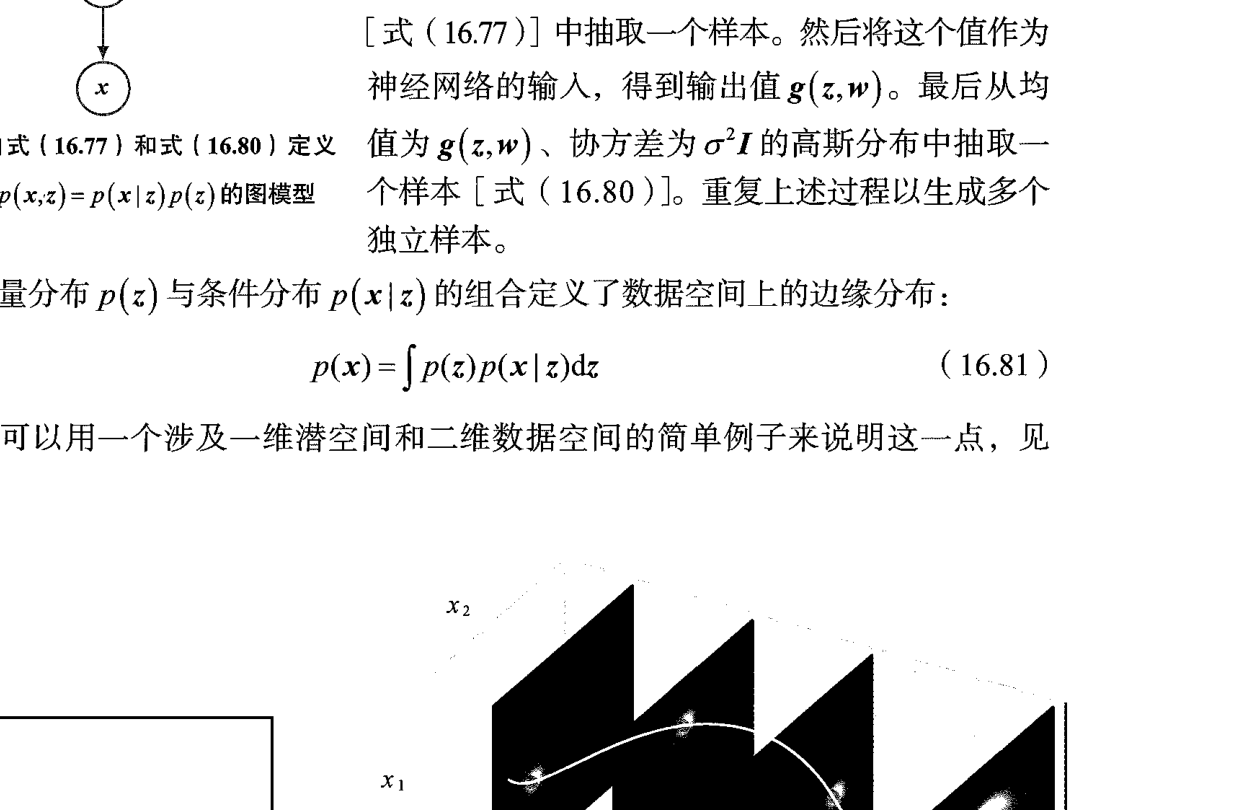
\includegraphics[width=0.85\textwidth]{ch16-fig16.13-nonlinear-lvm.png}
\caption{一个涉及一维潜空间和二维数据空间的非线性潜变量模型的示意图。(a)~潜空间中的先验分布由零均值、单位方差的高斯分布给出；(b)~最左侧的三个图显示了不同 $\bm{z}$ 值下的高斯条件分布 $p(\bm{x}|\bm{z})$ 的示例，最右侧的图显示了边缘分布 $p(\bm{x})$ 的示例。定义条件分布均值的非线性函数 $\bm{g}(\bm{z})$ 由 $g_1(z)=\sin(z)$ 和 $g_2(z)=\cos(z)$ 给出，条件分布的标准差由 $\sigma=0.3$ 给出。}
\label{fig:ch16-nonlinear-lvm}
\end{figure}

我们可以用一个涉及一维潜空间和二维数据空间的简单例子来说明这一点，如\cref{fig:ch16-nonlinear-lvm}所示。潜变量分布 $p(\bm{z})$ 与条件分布 $p(\bm{x}|\bm{z})$ 的组合定义了数据空间上的边缘分布：
\begin{align}
p(\bm{x})=\int p(\bm{z})p(\bm{x}|\bm{z})\,\mathrm{d}\bm{z}.
\label{align:ch16-nl-marginal}
\end{align}

其中神经网络 $\bm{g}(\bm{z},\bm{w})$ 的输出单元激活函数是线性的。生成式模型由 $\bm{z}$ 上的潜变量分布和 $\bm{x}$ 上的条件分布指定：
\begin{align}
p(\bm{x}|\bm{z},\bm{w})=\mathcal{N}(\bm{x}|\bm{g}(\bm{z},\bm{w}),\sigma^2\bm{I}).
\label{align:ch16-nl-conditional}
\end{align}

注意，从这个分布中独立抽取样本不仅简单而且效率高。首先使用标准方法从高斯分布中抽取一个样本，然后将这个值作为神经网络的输入，得到输出值 $\bm{g}(\bm{z},\bm{w})$。最后从均值为 $\bm{g}(\bm{z},\bm{w})$、协方差为 $\sigma^2\bm{I}$ 的高斯分布中抽取一个样本。

\subsection{似然函数}\label{subsection:ch16-似然函数}

我们已经看到从这个非线性潜变量模型中抽取样本是很容易的。假设我们希望通过最大化似然函数来拟合观测到的数据集。可以通过对 $\bm{z}$ 进行积分并使用概率的加和法则和乘积法则来得到似然值：
\begin{align}
p(\bm{x}|\bm{w})=\int p(\bm{x}|\bm{z},\bm{w})p(\bm{z})\,\mathrm{d}\bm{z}.
\label{align:ch16-nl-likelihood}
\end{align}

尽管积分内部的两个分布都是高斯分布，但由神经网络定义的高度非线性函数 $\bm{g}(\bm{z},\bm{w})$ 却使得积分在解析上是不可处理的。一种计算似然函数的方法是从潜空间分布 $p(\bm{z})$ 中抽取 $K$ 个样本，并用这些样本来近似式\eqref{align:ch16-nl-likelihood}，从而得到
\begin{align}
p(\bm{x}|\bm{w})\approx\frac{1}{K}\sum_{k=1}^{K}p(\bm{x}|\bm{z}^{(k)},\bm{w}),\qquad \bm{z}^{(k)}\sim p(\bm{z})
\label{align:ch16-mc-likelihood}
\end{align}

这将 $\bm{z}$ 的分布表示为具有固定混合系数 $1/K$ 的高斯混合分布。当样本数量趋于无穷时，该方法给出了真实的似然函数。然而，实际训练中所需的 $K$ 值通常会大得不切实际。

为什么会这样？考虑三个手写数字图像的例子。假设图~(a)~代表我们希望计算似然函数的向量 $\bm{x}$。如果一个训练好的模型生成了图~(b)，我们会认为这是一个比较差的模型，因为这个图像并不是数字"2"的一个很好的表示，所以应该被赋予一个更低的似然值。相反，图~(c)~是通过将图~(a)~中的数字向下和向右移动 $0.5$ 个像素获得的，是数字"2"的一个很好的表示，因此应该被赋予一个更高的似然值。由于是高斯分布，似然函数与网络输出和数据向量 $\bm{x}$ 之间负平方距离的指数成正比。如果方差参数 $\sigma^2$ 设置得足够小，使得图~(b)~具有低似然值，那么图~(c)~就会有更低的似然值。即使模型在生成数字方面做得很好，我们也必须抽取极大量的 $\bm{z}$ 样本，才能找到一个足够接近图~(a)~的样本。

然而，这个框架将零概率密度赋予那些不完全位于流形上的任何数据向量，这对基于梯度的学习算法是一个问题，因为对于真实的数据集，似然函数在每一个数据点都将为零，并且对于小的 $\bm{w}$ 变化将保持不变。为了解决这个问题，我们使用之前用于解决回归和分类问题的策略，定义了整个数据空间上的条件分布，其参数由神经网络的输出决定。例如，如果 $\bm{x}$ 是连续变量的一个向量，则可以选择条件分布为高斯分布。

\subsection{离散数据}\label{subsection:ch16-离散数据}

如果观测到的数据集包含独立的二进制变量，则可以使用以下形式的条件分布：
\begin{align}
p(\bm{x}|\bm{z},\bm{w})=\prod_{i=1}^{D}\mu_i(\bm{z},\bm{w})^{x_i}(1-\mu_i(\bm{z},\bm{w}))^{1-x_i}
\label{align:ch16-binary-conditional}
\end{align}
其中 $\mu_i(\bm{z},\bm{w})=\sigma(a_i(\bm{z},\bm{w}))$ 是输出单元 $i$ 的激活值，激活函数 $\sigma(\cdot)$ 由逻辑斯谛~sigmoid~函数给出，$a_i(\bm{z},\bm{w})$ 是输出单元 $i$ 的预激活值。类似地，对于独热编码（one-hot encoded）的分类变量，可以使用多项式分布：
\begin{align}
p(\bm{x}|\bm{z},\bm{w})=\prod_{i=1}^{D}\operatorname{softmax}(\bm{a}(\bm{z},\bm{w}))^{x_i}
\label{align:ch16-categorical-conditional}
\end{align}

我们还可以通过构造相关条件分布的乘积来考虑离散变量和连续变量的组合。

在实际应用中，连续变量通常以离散值表示，例如在图像中，红色、绿色和蓝色通道的强度可能取自~8~位二进制数字所能表示的数值集 $\{0,\cdots,255\}$。当我们采用基于深度神经网络的高度灵活模型时，这可能会导致一个问题：如果密度坍塌到一个或多个离散值上，似然函数就有可能变为零，导致异常解。这个问题可以通过使用一种称为去量化（dequantization）的技术来解决，该技术涉及向变量添加噪声，这些噪声在连续离散值之间的区域内通常是均匀分布的。训练集的去量化就是用随机抽取的样本替换每个观测值，这些样本来自与特定离散值相关联的连续分布。采用这种方法，模型找到异常解的可能性就会降低。

\subsection{构建生成式模型的四种方法}\label{subsection:ch16-四种生成模型}

我们已经看到，基于深度神经网络的非线性潜变量模型提供了一个高度灵活的框架来构建生成式模型。由于神经网络变换的普适性，这些模型原则上能够以高精度近似任何期望的分布。此外，一旦训练好，这些模型还可以使用一种高效、非迭代的过程从分布中生成样本。然而，我们也面临着一些与训练此类模型相关的挑战，迫切需要找到比线性模型更复杂的方法。业内已经提出了不少方法，每种方法都有自身的优势和局限性，它们大致可以分为以下四种：

\begin{enumerate}
\item 基于生成对抗网络（Generative Adversarial Network, GAN）（见第~17~章）放宽"网络映射必须是可逆的"这一要求，允许潜空间的维度低于数据空间的维度。这里也放弃了似然函数的概念，引入了第二个神经网络，其功能是为生成网络提供训练信号。由于缺乏明确定义的似然函数，训练过程可能不稳定，但一旦训练完成，就很容易从模型中生成样本，并且所得结果的质量也高。

\item 变分自编码器（Variational AutoEncoder, VAE）（见第~19~章）也使用了第二个神经网络，其作用是近似潜变量的后验分布，从而允许计算似然函数的近似值。与~GAN~相比，其能使训练更为稳健，而且能直接从训练好的模型中采样，但是要获得高质量的结果可能更困难。

\item 在标准化流（normalizing flow）（见第~18~章）中，将潜空间的维度设置为等于数据空间的维度，然后修改神经网络，使其变得可逆。"网络必须是可逆的"这一要求限制了其函数形式，但也使得无须近似就能计算似然函数，而且能进行高效采样。

\item 扩散模型（diffusion model）（见第~20~章）使用一个网络学习如何通过一系列去噪步骤将先验分布的样本转换为数据分布的样本。这在许多应用中带来了先进的性能，缺点是由于多次经历网络的去噪过程，采样成本可能较高。
\end{enumerate}

\section*{习题}\label{section:ch16-习题}
\addcontentsline{toc}{section}{习题}

\textbf{16.1}（$\star\star$）使用归纳法证明，将数据投影到 $M$ 维子空间以最大化投影数据的方差所定义的线性投影是由数据协方差矩阵 $\bm{S}$ 的 $M$ 个特征向量定义的，对应于 $M$ 个最大特征值。

\textbf{16.2}（$\star\star$）证明在满足正交性质[式\eqref{align:ch16-orthonormal}]的情况下，PCA~误差度量 $J$[由式\eqref{align:ch16-recon-error}给出]的最小值是在 $\bm{u}_j$ 为数据协方差矩阵 $\bm{S}$ 的特征向量时获得的。

\textbf{16.3}（$\star$）假设式\eqref{align:ch16-highdim-back}定义的特征向量 $\bm{v}$ 具有单位长度，验证这些特征向量已归一化至单位长度。

\textbf{16.4}（$\star$）假设在概率~PCA~模型中将零均值、单位协方差的潜空间分布[式\eqref{align:ch16-prior-z}]替换为一般形式的高斯分布 $\mathcal{N}(\bm{z}|\bm{m},\bm{\Sigma})$。通过重新定义模型的参数，证明这种替换会使得任意有效的 $\bm{m}$ 和 $\bm{\Sigma}$ 都无法改变观测变量边缘分布 $p(\bm{x})$ 的形式。

\textbf{16.6}（$\star\star$）利用一般高斯分布的均值和协方差公式，推导概率~PCA~模型中边缘分布 $p(\bm{x})$ 的结果[式\eqref{align:ch16-marginal-gauss}]。

\textbf{16.7}（$\star$）绘制~16.2~节描述的概率~PCA~模型的有向图，并将观测变量 $\bm{x}$ 的各个组成部分明确显示为单独的节点。验证概率~PCA~模型具有与朴素贝叶斯模型相同的独立结构。

\textbf{16.8}（$\star\star$）利用线性--高斯模型的结果，证明概率~PCA~模型的后验分布 $p(\bm{z}|\bm{x})$ 可以由式\eqref{align:ch16-post-mean}给出。

\textbf{16.9}（$\star$）验证对概率~PCA~模型的对数似然函数[式\eqref{align:ch16-ppca-nll2}]关于参数 $\bm{\mu}$ 进行最大化会得到结果 $\bm{\mu}=\bar{\bm{x}}$，其中 $\bar{\bm{x}}$ 是数据向量的均值。

\textbf{16.10}（$\star\star$）通过计算对数似然函数对参数 $\bm{\mu}$ 的二阶导数，证明驻点 $\bm{\mu}=\bar{\bm{x}}$ 代表唯一的最大值。

\textbf{16.11}（$\star\star$）证明当 $\sigma^2\rightarrow 0$ 时，概率~PCA~模型的后验均值相当于对主子空间的正交投影，这与传统~PCA~模型的结果一致。

\textbf{16.12}（$\star\star$）对于 $\sigma^2>0$，证明概率~PCA~模型中的后验均值会相对于正交投影向原点移动。

\textbf{16.13}（$\star\star$）证明在概率~PCA~下，根据传统~PCA~的最小二乘投影成本，数据点的最优重建由式\eqref{align:ch16-recon-ppca}给出。

\textbf{16.14}（$\star$）概率~PCA~模型中协方差矩阵的独立参数数量由式\eqref{align:ch16-cov-c}给出。证明对于 $M=D-1$，独立参数的数量与一般高斯分布中的相同；而对于 $M=0$，独立参数的数量与各向同性协方差高斯分布相同。

\textbf{16.15}（$\star$）推导出\cref{subsection:ch16-因子分析}描述的因子分析模型中独立参数数量的计算表达式。

\textbf{16.16}（$\star\star$）证明\cref{subsection:ch16-因子分析}描述的因子分析模型不随潜空间坐标旋转而变化。

\textbf{16.17}（$\star\star$）考虑一个线性--高斯潜变量模型，它具有潜空间分布 $p(\bm{z})=\mathcal{N}(\bm{z}|\bm{0},\bm{I})$ 和观测变量的条件分布 $p(\bm{x}|\bm{z})=\mathcal{N}(\bm{x}|\bm{W}\bm{z}+\bm{\mu},\bm{\Psi})$。对数据变量进行非奇异线性变换 $\bm{x}\rightarrow\bm{A}\bm{x}$，其中 $\bm{A}$ 是一个 $D\times D$ 矩阵。证明在两种情况下模型的形式得以保留：(i) $\bm{A}$ 是对角矩阵且 $\bm{\Psi}$ 也是对角矩阵（对应于因子分析）；(ii) $\bm{A}$ 是正交矩阵且 $\bm{\Psi}$ 与单位矩阵成比例（对应于概率~PCA）。

\textbf{16.18}（$\star$）验证连续潜变量模型对数似然函数可以写成两项之和[式\eqref{align:ch16-elbo}]，这两项分别由式\eqref{align:ch16-elbo-def}和式\eqref{align:ch16-kl}定义。

\textbf{16.19}（$\star$）证明对于一组独立同分布数据，证据下界（ELBO）可以采用式\eqref{align:ch16-elbo-iid}的形式。

\textbf{16.21}（$\star\star$）通过最大化式\eqref{align:ch16-q-ppca}给出的完整数据对数似然函数的期望来推导概率~PCA~模型的~M~步骤方程[式\eqref{align:ch16-m-step-w}]和[式\eqref{align:ch16-m-step-sigma}]。

\textbf{16.22}（$\star\star\star$）概率~PCA~的一个优点是，它可以应用于某些值缺失的数据集，前提是这些值是随机缺失的。在这种情况下，推导出最大化概率~PCA~模型似然函数的~EM~算法。

\textbf{16.25}（$\star\star$）给出因子分析模型的完整数据对数似然函数的期望的表达式，从而导出相应的~M~步骤方程[式\eqref{align:ch16-fa-m-w}]和[式\eqref{align:ch16-fa-m-psi}]。

\textbf{16.26}（$\star\star$）通过考虑二阶导数，证明\cref{subsection:ch16-因子分析}讨论的因子分析模型的对数似然函数相对于参数 $\bm{\mu}$ 的唯一驻点是由式\eqref{align:ch16-mean}定义的样本均值给出的。此外，证明这个驻点是一个最大值。

\end{document}
